% ================================================================================
\documentclass{article}
\pagestyle{plain}
\usepackage{fullpage}
% ================================================================================
%\usepackage[left=1in,right=1in, top=1.2in,bottom=1.2in]{geometry}
%\usepackage{times}
\usepackage{amssymb,amsthm,latexsym,amsmath,epsfig,pgf}

\usepackage{graphicx}
\usepackage{comment}
\usepackage{url}
\usepackage{hyperref}

\usepackage{blkarray}
\usepackage{tikzsymbols}

\usepackage[T1]{fontenc}
\usepackage[utf8]{inputenc}

\usepackage{blindtext}

\usepackage[nottoc,notlot,notlof]{tocbibind}
% ================================================================================
\usepackage{listings}
\lstset{
    %basicstyle=\small\ttfamily,
    frame=single,
    language=C,
    escapechar=|,
    numbers=left,
    stepnumber=1,
    %numbersep=-10pt,
    morekeywords={datatype, irrational, string, rule, list, list2D, new, node, node_T, node_Tstring, listnumber, fixedint, map, and, elseif, in, empty, pt}
}
% ================================================================================
\usepackage{algorithmicx}
\usepackage{algpseudocode}
\usepackage{algorithm}

\algnewcommand\algorithmicinput{\textbf{Input:}}
\algnewcommand\Input{\item[\algorithmicinput]}

\algnewcommand\algorithmicoutput{\textbf{Output:}}
\algnewcommand\Output{\item[\algorithmicoutput]}
% ================================================================================
\newtheorem{theorem}{Theorem}[section]
\newtheorem*{theorem A}{Theorem A}
\newtheorem*{theorem B}{N\"olker's Theorem}
\newtheorem{lemma}{Lemma}[section]
\newtheorem{proposition}{Proposition}[section]
\newtheorem{corollary}{Corollary}[section]
\newtheorem{definition}{Definition}
\newtheorem{problem}{Problem Statement}
\newtheorem{example}{Example}
\newtheorem{step}{Step} \setcounter{step}{-1}
\newtheorem*{question}{Question}
\newtheorem {conjecture}{Conjecture}
\theoremstyle{remark}
\newtheorem{remark}{Remark}[section]
\theoremstyle{remark}
\newtheorem{remarks}{Remarks}
% ================================================================================
\begin{document}
% ================================================================================
\title{Notes: The (maximum) independent set problem (MISP) on Riemannian manifolds of higher dimensions}
% ================================================================================
\author{Carolin Z\"obelein\thanks{The author believes in the importance of the independence of research and is funded by the public community. If you also believe in this values, you can find ways for supporting the author's work here: \url{https://research.carolin-zoebelein.de/funding.html}, Email: \href{mailto:contact@carolin-zoebelein.de}{\texttt{contact@carolin-zoebelein.de}}, PGP: D4A7 35E8 D47F 801F 2CF6 2BA7 927A FD3C DE47 E13B, \url{https://research.carolin-zoebelein.de}, CV availabe at \url{https://research.carolin-zoebelein.de/files/cv_longversion.pdf}, \Cooley}}
% ================================================================================
\date{October 14, 2020}   %\date{\today}
% ================================================================================
\maketitle
% ================================================================================
%\begin{center}
%    DRAFT
%\end{center}
% ================================================================================
\begin{abstract}
    We consider the determination of (maximum) independent sets of arbitrary graphs with the help of higher dimensional tensor based representations and subgraph decomposition by weighted based introduction of virtual edges. Finally, we do a comparison of our algorithm with a similiar one given by Tarjan in \textit{Decomposition by clique separators}. In contrast to Tarjan's algorithm, we propose an algorithm which offers the possibility to choose the atom subgraphs freely instead of handling mandatory atom subgraphs given by a decomposition.
\end{abstract}
% ================================================================================
\providecommand{\keywords}[1]{\small{\textbf{\textit{Keywords:}} #1}}
\providecommand{\Classification}[1]{\small{\textbf{\textit{ACM Subject Classes:}} #1}}

\begin{flushleft}
    \keywords{Maximum Independent Sets, Independent Sets, Graphs, Graph Theory, Riemannian Manifolds, Higher Dimensions, Tensors}\\
    %\Classification{}
\end{flushleft}
% ================================================================================
\tableofcontents
% ================================================================================
% --------------------------------------------------------------------------------
\section*{Preamble}
\label{s:preamble}
% --------------------------------------------------------------------------------
The following content is a sketch for discussion purposes only, without warranty for mathematical completeness.
% ================================================================================
% --------------------------------------------------------------------------------
\section{Basic definitions}
\label{s:basicdefinitions}
% --------------------------------------------------------------------------------
Given an \underline{undirected} and \underline{unweighted} graph $G = \left(V, E\right)$, by a \underline{finite} set of \underline{vertices} $V$ and a set of \underline{edges} $E := \{ e_{k} := \left(v_{i}, v_{j}\right) \in V^{2}\}$ on a \underline{Riemannian manifold} $M$ of $\mathbb{R}^{dim}$ with $dim := max\{ deg\left(v_{i}\right) \}$, $\forall \, v_{i} \in V$ of $G\left(V\right)$.

\vspace{0.3cm}
For two vertices $x$ and $y$, we write $x \sim y$ if they are connected by an edge. We say \underline{y is a neighbor of x} and write $N\left(x\right) := \{ y \in V \, : \, y \sim x \}$ for the \underline{set of all neighbors of x}.

\vspace{0.3cm}
The number of vertices connecting to x, is called the \underline{degree} of $x$ and denoted by \underline{$deg\left(x\right)$}. Since $G\left(V\right)$ is finite, by $|V| < \infty$, also $deg\left(x\right)$ is finite. The maximum possible degree of a vertex in a finite graph is $deg_{max}\left(x\right) := |V| - 1$.

\vspace{0.3cm}
We call a graph $G\left(V\right)$ \underline{connected} if for all two vertices $x$ and $y$ in $V$, there exists a finite number of vertices $\{ v_{i} \}_{i=1}^{m}$ in $V$, satisfying that $v_{1} := x$, $v_{m} := y$ and $v_{i}$ is connected to $v_{i+1}$, $\forall \, i = 1,2,\dots, m-1$.


\vspace{0.3cm}
\begin{remark}
    Without loss of generality, as long not other mentioned, we assume that all in the following considered graphs are \underline{connected graphs} (We introduce not-connected cases, later).
\label{remark:connectedgraphs}
\end{remark} 

\vspace{0.3cm}
An \underline{Eulerian cycle} in an undirected graph is a cycle that uses each edge exactly once. A graph which owns such a cycle is called \underline{Eulerian}. If $G\left(V\right)$ is a \textit{connected} graph, then the following statements are equivalent:

\begin{enumerate}
    \item $G$ is Eulerian
    \item Every vertex $v \in V$ of $G$ have an even degree $deg\left(v\right)$
    \item The set $E$ of $G$ is the set union of all edges of pairwise disjunct cycles
\label{enum:euleriancycle}
\end{enumerate}

This was proofed by Hierholzer \cite{hierholzer1873moglichkeit}.

\vspace{0.3cm}
$\Rightarrow$ A graph $G$ which has \underline{only vertices} with \underline{even degrees} is \underline{Eulerian}.

\vspace{0.3cm}
\begin{remark}
    Without loss of generality, as long not other mentioned, we assume that all in the following considered graphs are \underline{Eulerian graphs} ($\Rightarrow$ All vertices have even degree), (We introduce not-Eulerian cases, later).
\label{remark:euleriangraphs}
\end{remark}

\vspace{0.3cm}
We define a \underline{vertex path}, connecting two vertices $x,y \in V$ by $S := \left[ c_{0},c_{1}, \cdots, c_{n-2}, c_{n-1} \right]$ or short $ = c_{0}c_{1}c_{2}\cdots c_{n-2}c_{n-1}$ with $c_{0} := x$ and $c_{n} := y$ and $c_{i} \sim c_{i+1}$ for each $i = 0,1,\cdots,n-2$.

\vspace{0.3cm}
We denote an \underline{Eulerian cycle} of $G$ by $S_{E} := \left[b_{0},b_{1}, \cdots, b_{n-2}, b_{n-1}\right]$ or short $ = b_{0}b_{1}\cdots b_{n-2}b_{n-1}$ with \underline{length $l\left(S_{E}\right) = |E| + 2$}, \underline{$b_{0} = b_{n-1}$}, and each edge $b_{i} \sim b_{i+1}$ appears \textit{exactly ones}.

\vspace{0.3cm}
Given an Eulerian graph $G$, its belonging Eulerian cycle is not unique. It can exist more than one Eulerian cycles $S_{E}$ of $G$.

\vspace{0.3cm}
Assume, we know one Eulerian cycle $S_{E,1}$ of $G$. We can derive further Eulerian cycles $S_{E, k > 1}$ of $G$ by the set of systematically, cyclically permutations $\pi_{k}$ of vertices of $S_{E,1}$ with

\begin{equation*}
    \begin{split}
         \{ \pi_{k} \, : \,     & \left[ b_{0}, b_{1}, b_{2} \cdots, b_{n-3}, b_{n-2}, b_{n-1} \right]\\
            \rightarrow         & \left[ b_{1}, b_{2}, b_{3} \cdots, b_{n-2}, b_{n-1}, b_{0} \right]\\
            \rightarrow         & \left[ b_{2}, b_{3}, b_{4} \cdots, b_{n-1}, b_{0}, b_{1} \right]\\
            \cdots\\
            \rightarrow         & \left[ b_{n-1}, b_{0}, b_{1}, \cdots, b_{n-4}, b_{n-3}, b_{n-2} \right] \}
    \label{eq:euleriancycles}
    \end{split}
\end{equation*}

All this Eulerian cycles are in fact the same Eulerian cycle.

\vspace{0.3cm}
Given an Eulerian cycle $S_{E}$ of an Eulerian graph $G$. Each vertex $v_{i} \in V$ of $G$ appears exactly $deg\left(v_{i}\right)/2$ times within the Eulerian cycle $S_{E}$, except the vertex $v_{k} := b_{0} = b_{n-1}$, which appears exactly $deg\left(v_{k}\right)/2 + 1$ times within the Eulerian cycle $S_{E}$.

\vspace{0.3cm}
We call an Eulerian cycle representation a \underline{disruptive bit string} representation, if we write for an Eulerian cycle $S_{E}$, $S_{E}^{N-1^\prime} := \left[b^{\prime}_{N-1}, b^{\prime}_{N-2}, \cdots, b^{\prime}_{1}, b^{\prime}_{0}\right]$ or short $ = b^{\prime}_{N-1}b^{\prime}_{N-2} \cdots b^{\prime}_{1}b^{\prime}_{0}$ with $b^{\prime}_{i} \in \{ 0, 1 \}$, length $l\left(S^{N-1^{\prime}}_{E}\right) = |E| + 2 = N$, $i \sim i + 1$, which satisfies the following properties:

\begin{enumerate}
    \item Direct consecutive bits $b^{\prime}_{i}b^{\prime}_{i-1}$ are allowed to have the bit patterns $00$, $01$ and $10$. The bit pattern $11$ be prohibit.

    \item A \underline{coupling} $c$ of bits $b^{\prime} \in S^{N-1^\prime}_{E}$ be given by $c_{\alpha := i, \dots, j} := \{ \left(b_{i}, \dots, b_{j}\right) \, | \, b_{i} = \dots = b_{j}, \, \forall \, i,j \, : \, i \neq j \}$ and $|c_{\alpha := i, \dots, j}| \geq 2$. Furthermore, for all couplings $c_{\alpha}$ and $c_{\beta}$, we have $c_{\alpha} \cap c_{\beta} = \emptyset$. We will denote all bits $b^{\prime}$ which belong to the same coupling $c$ by $b^{c^\prime}$. The bit string $S^{N-1^\prime}_{E}$ consists of at least one coupling of bits, which is $c_{N-1,0} := \left(b^{\prime}_{N-1}, b^{\prime}_{0}\right)$.
\label{enum:distruptivebitstringrep}
\end{enumerate}


\vspace{0.3cm}
\begin{problem}[Maximization of the number of $1$s in $S^{N-1^{\prime}}_{E}$]
    Given a disruptive bit string $S^{N-1^\prime}_{E}$ by its total length $N \in \mathbb{N}$ and a fixed set of gien couplings $c \in \mathcal{C}$. We ask for the values of $S^{N-1^\prime}_{E}$, so that the number of $1$s gets maximized in $S^{N-1^\prime}_{E}$ if we count $1$s of bits belonging to the same coupling only once within each coupling.
\label{problem:maximizationof1s}
\end{problem}


\vspace{0.3cm}
\begin{remark}
    The given problem statement describes the question of the \underline{\textbf{M}aximum \textbf{I}ndependent \textbf{S}et \textbf{P}roblem} (short: MISP).
\label{remark:MISP}
\end{remark}
% --------------------------------------------------------------------------------
\section{Decomposition}
\label{s:decomposition}
% --------------------------------------------------------------------------------
Given an undirected and unweighted graph $G\left(V\right)$ on a Riemannian manifold $M$ of $\mathbb{R}^{dim}$ with $dim := max\{ deg\left(v_{i}\right) \}$, $\forall \, v_{i} \in V$ of $G\left(V\right)$.

\vspace{0.3cm}
Consider a vertices coordination of vector $\vec{v} = \left(v_{1}, v_{2}, \dots, v_{n}\right)^{T}$, $\forall \, v_{i} \in V$, $n := |V|$. The unity norm between two direct consecutive vertices of $V$ according their ascending index order, be $1$ ($d\left(v_{i}, v_{i+1}\right) = 1$).

\vspace{0.3cm}
The edges of $G\left(V\right)$ on $\mathbb{R}^{dim}$ can be represented by an $\mathbb{R}^{dim}$ tensor structure, called \underline{adjacence tensor} $T$. $T$ is given by $\underbrace{\vec{v} \otimes \vec{v} \otimes \vec{v} \otimes \cdots \otimes \vec{v}}_{\mathrm{dim-times}}$.

\vspace{0.3cm}
If it exists a mapping $\phi \, : \, \mathbb{R}^{dim} \rightarrow \mathbb{R}^{2}$ of $G\left(V\right)$, then we call $G\left(V\right)$ a \underline{flat surface graph} in terms of $\phi$ and $T$ of the mapped flat surface graph equals the well known classical adjacence matrix representation of $G\left(V\right)$\footnote{\underline{Attention}: Flat surface \textbf{doesn't} mean planar. It only means its structure can be represented by a well known 2D-adjacence matrix!}.

\vspace{0.3cm}
The \textit{innner concatenation} $\circ$ of $T$ entries is denoted by $t_{\underbrace{ijk\cdots}_{\mathrm{dim-factors}}} := \underbrace{v_{i} \circ v_{j} \circ v_{k} \circ \dots}_{\mathrm{dim-factors}}$ or short $v_{i}v_{j}v_{k} \cdots$ and called \underline{edge conservation}. It is defined as follows:

\begin{enumerate}
    \item If there exists a mapping $\phi \, : \, \mathbb{R}^{dim} \rightarrow \mathbb{R}^{2}$ of $G\left(V\right)$, so that $G\left(V\right)$ can be considered as a flat surface graph in terms of $\phi$, then we can denote each entry of $T^{V}_{dim=2}$ ($T^{V}_{dim=2}$ being the $dim = 2$ tensor of a flat surface graph $G\left(V\right)$ in terms of $\phi$) by $t_{ij} := v_{i}v_{j}$, $i,j \in \{ 1,2,\dots, n \}$, which describes the edge characteristics between the two vertices $v_{i}$ and $v_{j}$ by

    \begin{equation*}
        t_{ij} := edge\left(i,j\right) = 
        \begin{cases}
            1   & \text{if there exists an edge between } v_{i} \text{ and } v_{j}\\
            0   & \text{otherwise}
        \end{cases}
    \label{eq:edge2}
    \end{equation*}

    \item Be $G\left(V\right)$ a graph on a $\mathbb{R}^{dim}$ Riemannian manifold $M$. The edge conservation of $T^{V}_{dim}$ for each entry is given by $t_{i_{1}, i_{2}, \dots, i_{dim}}$, $i_{1}, i_{2}, \dots, i_{dim} \in \{ 1,2, \dots, n \}$, with $t_{i_{1}, i_{2}, \dots, i_{dim}} := v_{i_{1}} v_{i_{2}} \cdots v_{i_{dim}}$, which describes the edge characteristics between the vertices $\{ v_{i_{1}}, v_{i_{2}}, \dots, v_{i_{dim}} \}$ by 

    \begin{equation*}
        t_{i_{1}i_{2}\dots i_{dim}} := edge\left(i_{1},i_{2},\dots,i_{dim}\right) = 
        \begin{cases}
            1   & \left(\star\right) \text{ see explanation beneath}\\
            0   & \left(\star\right) \text{ see explanation beneath}
        \end{cases}
    \label{eq:edgeDim}
    \end{equation*}

    $\left(\star\right)$ Consider a graph $G\left(V\right)$ on $\mathbb{R}^{dim > 2}$ on a Riemannian manifold $M$. We define an edge of an higher dimensional case > 2 recursively in the following way:

    \begin{enumerate}
        \item We assume that for dimension \underline{$dim$} $edge\left(i_{1}, i_{2}, \dots, i_{dim}\right)$ defines an edge characteristic between the vertices $v_{i_{1}}, v_{i_{2}}, \cdots v_{i_{dim}}$.

        \item Then the edge characteristic for dimension \underline{$dim + 1$}, $edge\left(i_{1}, i_{2}, \dots, i_{dim}, i_{dim + 1}\right)$ defines an edge characteristic between the vertices $v_{i_{1}}, v_{i_{2}}, \dots, v_{i_{dim}}, v_{i_{dim + 1}}$ by $edge\left(i_{1}, i_{2}, \dots, i_{dim}, i_{dim + 1}\right)$ induced an edge characteristic on the concatenation of the edge characteristic $edge\left(i_{1}, i_{2}, \dots, i_{dim}\right)$ with $v_{i_{dim + 1}}$, $edge\left(i_{1}, i_{2}, \dots, i_{dim}, i_{dim + 1}\right) := edge\left(edge\left(i_{1}, i_{2}, \dots, i_{dim}\right), i_{dim + 1}\right)$.
    \label{enum:edgesdim+1case}
    \end{enumerate}
\label{enum:edges}
\end{enumerate}


\vspace{0.3cm}
$\rightarrow$ We consider subgraphs, at first.

\vspace{0.3cm}
Be $A$ a subset of $V$, $A \subseteq V$, such that $G\left(A\right)$ be a \underline{connected subgraph} of $G\left(V\right)$ with size $|A| \geq 1$.

\vspace{0.3cm}
We denote the graph which is given by the remaining vertices $V \setminus A$ by $G\left(V - A\right)$.

\vspace{0.3cm}
The subset $D$ of vertices $D \subseteq V$, called \underline{influencers of $A$}, denoted by $D_{A}$ (or only $D$ if it is clear which susbset we are talking about because of the context), be the set of all vertices $d_{i}$ with:


\begin{equation*}
    \begin{split}
        \{ \forall d_{i} \in V \, : \,  &\exists \left(edge\left(d_{i}, x_{l}\right) \wedge edge\left(d_{i}, a_{k}\right)\right), \text{with } x_{l} \in \left(V \setminus A\right) \text{ and } a_{k} \in A,\\
                    \text{or} \quad     &\exists \left(edge\left(d_{i}, a_{k}\right) \wedge edge\left(d_{i}, a_{k^{\prime}}\right)\right), \text{with } a_{k}, a_{k^{\prime}} \in A \}
    \label{eq:influencers}
    \end{split}
\end{equation*}


\vspace{0.3cm}
Now, we want to analyse a decomposition of $G\left(V\right)$ with similarities to the MIS algorithm proposed by Tarjan in \cite{tarjan1985decomposition} (section: '3.4. Maximum independent sets').

\vspace{0.3cm}
We consider a set $\mathcal{A}$ of connected subgraphs $G\left(A_{i}\right)$ of $G\left(V\right)$ by $\mathcal{A} := \{ A_{i} \}$ with pairwise $A_{i} \cap A_{j} = \emptyset$ and $\mathcal{A} \neq \emptyset$. Furthermore, there exists no edege $\left(a_{i}, a_{j}\right)$, $a_{i} \in A_{i}$ and $a_{j} \in A_{j}$.

\vspace{0.3cm}
We denote the MIS of $G\left(\mathcal{A}\right)$ by $I^{\prime}$.

\vspace{0.3cm}
We introduce a \underline{split function} $sp$ which splits a graph $G\left(V\right)$ into $G\left(\mathcal{A}\right)$ and $G^{\prime \prime} := G\left(V - \mathcal{A}\right)$.

\vspace{0.3cm}
During splitting, $sp$ induces over the \underline{impact} $imp\left(V - \mathcal{A}\right)$ a \underline{dimension recalibration} on $G\left(V - \mathcal{A}\right)$ by $sp \rightarrow imp\left(V - \mathcal{A}\right)$, $\mathbb{R}^{dim} \rightarrow \mathbb{R}^{dim^{\prime}}$, with $dim^{\prime} := max\{ deg\left(v_{i}\right) \}$, $\forall \, v_{i} \in \left(V  \setminus \mathcal{A}\right)$, and an \underline{edge influence} $inf$ on the graph $G\left(V - \mathcal{A}\right)$ in the following way:

\begin{enumerate}
    \item $inf$ introduces a \underline{new weighted virtual edge} ($e^{w} := \left(d_{i}, d_{j}\right)$) $e^{w}_{dim^{\prime}} = \left(e^{w}_{dim^{\prime} - 1}, d_{j}\right)$, $d_{j} \in D_{\mathcal{A}}$ \underline{and} $d_{k}$ of $e^{w}_{dim^{\prime} - 1}$ with $d_{k} \in D_{\mathcal{A}}$, $D_{\mathcal{A}}$ be our set of influencers of $\mathcal{A}$, on the graph $G\left(V - \mathcal{A}\right)$, if there exists a MIS \underline{size reducing influence} on $I^{\prime}$ of $G\left(\mathcal{A}\right)$, denoted by $inf\left(I^{\prime}, e^{w}\right)$, because of the establishing of the edge $e^{w}$ (if there not already existed that edge before).

    \item If there already existed that edge $e^{w} := \left(e^{w}_{dim^{\prime} - 1}, d_{j}\right)$ before, we don't change anything and call it a \underline{neutral}, $id$, influence.
\label{enum:newedge}
\end{enumerate}


\vspace{0.3cm}
We denote the \underline{new adjacence tensor} of $G\left(V - \mathcal{A}\right)$ by $T^{V - \mathcal{A}}_{dim^{\prime}}$ if we introduced \underline{weighted} virtual edges $e^{w}$ which give us the amount of negative changing of $I^{\prime}$ with $T^{V - \mathcal{A}}_{dim^{\prime}}$ entries of $e^{w}$'s with values $\leq -1$, $\forall \, e^{w}$ in $T^{V - \mathcal{A}}_{dim^{\prime}}$.

\vspace{0.3cm}
We identify edges in $T^{V - \mathcal{A}}_{dim^{\prime}}$ of $V \setminus \mathcal{A}$ with $edge\left(d_{i}, y_{k}\right)$ or $edge\left(y_{k}, y_{l}\right)$\footnote{This is for the flat surface graph case. In generally, we consider of course $edge\left(edge_{dim^{\prime} - 1}, y_{l}\right)$ with $d_{i}$ or $y_{k} \in edge_{dim^{\prime} - 1}$.}, $d_{i} \in D_{\mathcal{A}}$ and $y_{k}, y_{l} \in V \setminus \{ \mathcal{A} \cup D_{\mathcal{A}} \}$, with $d_{i} \sim y_{k}$ respectively $y_{k} \sim y_{l}$ as prohibit pattern '$11$' bit string connections and hence mark this edges in the weighted adjacence tensor $T^{V - \mathcal{A}}_{dim^{\prime}}$ with an entry value of '$-\infty$'.

\vspace{0.3cm}
We denote the so called \underline{standadized new adjacence tensor} of $G\left(V - \mathcal{A}\right)$ by $T^{\left(V - \mathcal{A}\right)^{\prime}}_{dim^{\prime}}$ in which we set all of the entry values of the weighted adjacence tensor $T^{V - \mathcal{A}}_{dim^{\prime}}$, which are $\neq 0$, to $1$.

\vspace{0.3cm}
Looking at the weighted adjacence tensor $T^{V - \mathcal{A}}_{dim^{\prime}}$, we want to give a short, sketchy, discussion regarding (maximum) independent sets.

\begin{enumerate}
    \item Tensor $T^{V - \mathcal{A}}_{dim^{\prime}}$ is symetrically according its dimensional diagonals. ($\Rightarrow$ for example $v_{1}v_{2}v_{3} = v_{1}v_{3}v_{2} = v_{2}v_{3}v_{1} = \cdots$)

    \item We call diagnonals of the form $\underbrace{v_{i_{1}} v_{i_{1}} v_{i_{1}} \cdots v_{i_{1}}}_{dim^{\prime}-times}$ 1-diagonal forms

    \item We don't have multiple edges. Means e.g. $v_{1}v_{2}v_{2} = v_{1}v_{2}$ with one edge between $v_{1}$ and $v_{2}$

    \item If we sum the values of $T^{V - \mathcal{A}}_{dim^{\prime}}$ entries, because of symmetry of $T^{V - \mathcal{A}}_{dim^{\prime}}$, we only sum entries of the valid symmetry area. Additionally, we have to take into account that during determing $T^{V - \mathcal{A}}_{dim^{\prime}}$, entries of diagonals are generated by multiple counting of changings. Hence, the sum of diagonal entries is gien by the norming to $-1$ over the number of diagonal entries over which we sum ($\left( \mathrm{sum} \ t_{diagonal}\right) 1/|\{ t_{diagonal} \} |$)

    \item Possibility discussion for finding maximum independent sets in $T^{\left(V - \mathcal{A}\right)^{\prime}}_{dim^{\prime}}$ for the example of a flat surface graph $G\left(V - \mathcal{A}\right)$ on $\mathbb{R}^{2}$.


    \vspace{0.3cm}
    \underline{Case 1} (see figure \ref{fig:case1}, $\left(\star\right)$ entries which are not given are $< -1$)\\

    \begin{figure}[ht]
	    \centering
        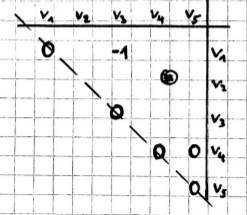
\includegraphics[width=0.33\textwidth]{images/case1.png}
	    \caption{Case 1}
	\label{fig:case1}
    \end{figure}

    $\rightarrow$ $\{ v_{4}, v_{5} \}$ IS of size $2$ on $G\left(V - \mathcal{A}\right)$\\
        $\Rightarrow$ $|I| = |I^{\prime}| + |IS| = |I^{\prime}| + 2$

    \vspace{0.3cm}
    $\rightarrow$ $\{ v_{1}, v_{3} \}$ set of size $2$ on $G\left(V - \mathcal{A}\right)$ but reducing the IS $I^{\prime}$ of $G\left(\mathcal{A}\right)$ by $-1$.\\
        $\Rightarrow$ $|I| = |I^{\prime}| - 1 + |set| = |I^{\prime}| - 1 + 2 = |I^{\prime}| + 1$

    \vspace{0.3cm}
    $\rightarrow$ $\{ v_{1} \}$ or $\{ v_{2} \}$ IS of size $1$ on $G\left(V - \mathcal{A}\right)$\\
        $\Rightarrow$ $|I| = |I^{\prime}| + |IS| = |I^{\prime}| + 1$

    \vspace{0.3cm}
    $\Rightarrow$ $\{ v_{4}, v_{5} \}$ leads us to the MIS of $G\left(V\right)$

    \vspace{0.3cm}
    $\Rightarrow$ In this case, we can determine the MIS of $G\left(V\right)$ by solving the MIS problem of the standardized adjacence tensor $T^{\left(V - \mathcal{A}\right)^{\prime}}_{dim^{\prime}}$.


    \vspace{0.3cm}
    \begin{remark}
        For each subgraph $A_{i}$ of $\mathcal{A}$ (for flat surface graphs) we can get maximal one $v_{i}v_{j} = 0$, with $v_{i} \neq v_{j}$, entry.
    \label{remark:cases}
    \end{remark}

    

    \vspace{0.3cm}
    \underline{Case 2} (see figure \ref{fig:case2})\\

     \begin{figure}[ht]
	    \centering
        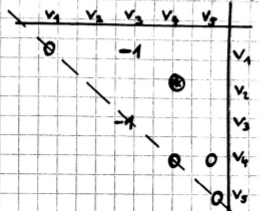
\includegraphics[width=0.33\textwidth]{images/case2.png}
	    \caption{Case 2}
	\label{fig:case2}
    \end{figure}

    $\rightarrow$ $\{ v_{4}, v_{5} \}$ IS of size $2$ on $G\left(V - \mathcal{A}\right)$\\
        $\Rightarrow$ $|I| = |I^{\prime}| + |IS| = |I^{\prime}| + 2$

    \vspace{0.3cm}
    $\rightarrow$ $\{ v_{1} \}$ IS of size $1$ on $G\left(V - \mathcal{A}\right)$\\
        $\Rightarrow$ $|I| = |I^{\prime}| + |IS| = |I^{\prime}| + 1$

    \vspace{0.3cm}
    $\rightarrow$ $\{ v_{1}, v_{3} \}$ set of size $2$ on $G\left(V - \mathcal{A}\right)$ but reducing the IS $I^{\prime}$ of $G\left(\mathcal{A}\right)$ by $- 1 - 1 = -2$.\\
        $\Rightarrow$ $|I| = |I^{\prime}| - 2 + |set| = |I^{\prime}| - 2 + 2 = |I^{\prime}|$

    \vspace{0.3cm}
    $\Rightarrow$ $\{ v_{4}, v_{5} \}$ leads us to the MIS of $G\left(V\right)$.

    \vspace{0.3cm}
    $\Rightarrow$ In this case, we can determine the MIS of $G\left(V\right)$ by solving the MIS problem of the standardized adjacence tensor $T^{\left(V - \mathcal{A}\right)^{\prime}}_{dim^{\prime}}$



    \vspace{0.3cm}
    \underline{Case 3} (see figure \ref{fig:case3})\\

     \begin{figure}[ht]
	    \centering
        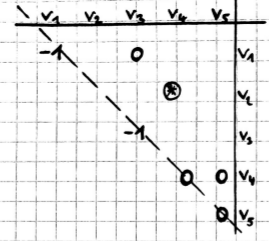
\includegraphics[width=0.33\textwidth]{images/case3.png}
	    \caption{Case 3}
	\label{fig:case3}
    \end{figure}

    $\rightarrow$ $\{ v_{3} \}$ or $\{ v_{1} \}$ set of size $1$ on $G\left(V - \mathcal{A}\right)$ but reducing the IS $I^{\prime}$ of $G\left(\mathcal{A}\right)$ by $-1$\\
        $\Rightarrow$ $|I| = |I^{\prime}| - 1 + |set| = |I^{\prime}| - 1 + 1 = |I^{\prime}|$

    \vspace{0.3cm}
    $\rightarrow$ $\{ v_{1}, v_{3} \}$ set of size $2$ on $G\left(V - \mathcal{A}\right)$ but reducing the IS $I^{\prime}$ of $G\left(\mathcal{A}\right)$ by $-1$ if $v_{1}$ and $v_{3}$ (like in our example) are elements of the same $D_{A_{i}}$, and $-2$ if $v_{1}$ and $v_{3}$ belong to different $D_{A_{i}} \neq D_{A_{j}}$.\\
        $\Rightarrow$ For our example, we get $|I| = |I^{\prime}| - 1 + |set| = |I^{\prime}| - 1 + 2 = |I^{\prime}| + 1$\\
            (else: $|I| = |I^{\prime}| - 2 + 2 = |I^{\prime}|$)

    \vspace{0.3cm}
    $\rightarrow$ $\{ v_{4}, v_{5} \}$ IS of size $2$ on $G\left(V - \mathcal{A}\right)$\\
        $\Rightarrow$ $|I| = |I^{\prime}| + |IS| = |I^{\prime}| + 2$

    \vspace{0.3cm}
    $\Rightarrow$ $\{ v_{4}, v_{5} \}$ leads us to the MIS of $G\left(V\right)$.

    \vspace{0.3cm}
    $\Rightarrow$ In this case, we can determine the MIS of $G\left(V\right)$ by solving the MIS problem of the standardized adjacence tensor $T^{\left(V - \mathcal{A}\right)^{\prime}}_{dim^{\prime}}$.



    \vspace{0.3cm}
    \underline{Case 4} (see figure \ref{fig:case4})\\

     \begin{figure}[ht]
	    \centering
        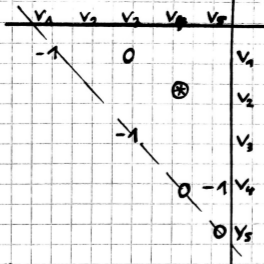
\includegraphics[width=0.33\textwidth]{images/case4.png}
	    \caption{Case 4}
	\label{fig:case4}
    \end{figure}

    $\rightarrow$ $\{ v_{3} \}$, $\{ v_{4} \}$ set of size $1$ on $G\left(V - \mathcal{A}\right)$ but reducing the IS $I^{\prime}$ of $G\left(\mathcal{A}\right)$ by $-1$.\\
        $\Rightarrow$ $|I| = |I^{\prime}| - 1 + |set| = |I^{\prime}| - 1 + 1 = |I^{\prime}|$

    \vspace{0.3cm}
    $\rightarrow$ $\{ v_{1}, v_{3} \}$ set of size $2$ on $G\left(V - \mathcal{A}\right)$ but reducing the IS of $I^{\prime}$ of $G\left(\mathcal{A}\right)$ by $-1$.\\
        $\Rightarrow$ $|I| = |I^{\prime}| - 1 + 2 = |I^{\prime}| + 1$

    \vspace{0.3cm}
    $\rightarrow$ $\{ v_{4} \}$ or $\{ v_{5} \}$ IS of size $1$ on $G\left(V - \mathcal{A}\right)$\\
        $\Rightarrow$ $|I| = |I^{\prime}| + |IS| = |I^{\prime}| + 1$

    \vspace{0.3cm}
    $\rightarrow$ $\{ v_{4}, v_{5} \}$ set of size $2$ on $G\left(V - \mathcal{A}\right)$ but reducing the IS $I^{\prime}$ of $G\left(\mathcal{A}\right)$ by $-1$.\\
        $\Rightarrow$ $|I| = |I^{\prime}| - 1 + |set| = |I^{\prime}| - 1 + 2 = |I^{\prime}| + 1$

    \vspace{0.3cm}
    $\Rightarrow$ We see, that in this case, we get the MIS of $G\left(V\right)$ with size $|I^{\prime}| + 1$ for: $\{ v_{1}, v_{3} \}$, $\{ v_{4} \}$, $\{ v_{5} \}$, $\{ v_{4}, v_{5} \}$

\label{enum:independentsetdiscussion}
\end{enumerate}


\vspace{0.3cm}
\underline{Discussion of case 4:}
\begin{enumerate}
    \item Assume we take the standardized adjacence tensor $T^{\left(V - \mathcal{A}\right)^{\prime}}_{dim^{\prime}}$. So, we have in figure \ref{fig:case4disitem1}:

        \begin{figure}[ht]
	        \centering
            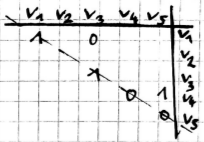
\includegraphics[width=0.33\textwidth]{images/discussionCase4Item1.png}
	        \caption{Discussion of case 4, item 1}
	        \label{fig:case4disitem1}
        \end{figure}
    
        \vspace{0.3cm}
        We get a MIS: $\{ v_{4} \}$ and $\{ v_{5} \}$\\
        $\Rightarrow$ We can derive the set $\{ v_{4}, v_{5} \}$ by having an additional look at our original weighted tensor $T^{V - \mathcal{A}}_{dim^{\prime}}$, by taking $v_{4}$ and $v_{5}$ and seeing that $v_{4}v_{5} = - 1$, so just a reducing by $-1$ by taking an addiontal vertex to $v_{4}$ (respectively taking an additional vertex to $v_{5}$). $\Rightarrow$ So, we get the same total size solution of $|I|$, $G\left(V\right)$, by $\{ v_{4}, v_{5} \}$

        \vspace{0.3cm}
        $\rightarrow$ $\{ v_{1}, v_{3} \}$ would be not find by a MIS solution of $G\left(V - \mathcal{A}\right)$. We only get it, if we notice that $v_{1}v_{3} = 0$ and that all diagonal entries of the participating vertices are $-1$ in $T^{V - \mathcal{A}}_{dim^{\prime}}$. So, we would also get this set of vertices.

        \vspace{0.3cm}
        $\rightarrow$ If we put all together, we get totally: $\{ v_{1}, v_{3} \} \cup \{ v_{4} \}$ and $\{ v_{1}, v_{3} \} \cup \{ v_{5} \}$ and $\{ v_{1}, v_{3} \} \cup \{ v_{4}, v_{5} \}$, all with the same total MIS size of $G\left(V - \mathcal{A}\right)$ by $|I| = |I^{\prime}| + 1 + 1 = |I^{\prime}| + 2$.

    \item Assume, we take the standardized adjacence tensor $T^{\left(V - \mathcal{A}\right)^{\prime}}_{dim^{\prime}}$, but set all diagonal entries to $0$ (see figure \ref{fig:case4disitem2}). We get the MIS $\{ v_{1}, v_{3} \}$ with $|I| = |I^{\prime}| + 2$ which is obvousily wrong.

        \begin{figure}[ht]
	        \centering
            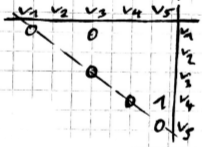
\includegraphics[width=0.33\textwidth]{images/discussionCase4Item2.png}
	        \caption{Discussion of case 4, item 2}
	    \label{fig:case4disitem2}
        \end{figure}

        \vspace{0.3cm}
        $\Rightarrow$ So it is necessary still to check the results in the original tensor $T^{\left(V - \mathcal{A}\right)^{\prime}}_{dim^{\prime}}$.

        \vspace{0.3cm}
        $\Rightarrow$ Furthermore, with an MIS algorithm on this tensor, here, we would not find $\{ v_{4} \}$, $\{ v_{5} \}$ and $\{ v_{4}, v_{5} \}$!
\label{enum:disccase4}
\end{enumerate}


\vspace{0.3cm}
We assume, that we are able to identify the MIS in $G\left(\mathcal{A}\right)$, which we denote by $I^{\prime}$.

\vspace{0.3cm}
We look again at the weighted adjacence tensor $T^{V - \mathcal{A}}_{dim^{\prime}}$.

\begin{enumerate}
    \item \underline{Case}:\\
        The MIS of $G\left(V - \mathcal{A}\right)$ is given by a set of vertice entries in $T^{V - \mathcal{A}}_{dim^{\prime}}$ in which all entries of the vertices of this set have value $0$.

        \vspace{0.3cm}
        $\Rightarrow$ We denote this MIS by $I^{\prime \prime}$ and recognize that the already known MIS of $G\left(\mathcal{A}\right)$ by \underline{$I^{\prime}$ \textbf{doesn't} get reduced} in its size.

        \vspace{0.3cm}
        $\Rightarrow$ The total MIS of $G\left(V\right)$ is given by: $I = I^{\prime} \cup I^{\prime \prime}$ and $I^{\prime \prime}$ in $T^{V - \mathcal{A}}_{dim^{\prime}}$ consists of only $0$ entries, so we have no participating edge in $I^{\prime \prime}$ (similar to the case: $I^{\prime \prime} \cap C = \emptyset$ in \cite{tarjan1985decomposition}).

    \item \underline{Case}:\\
        The MIS of $G\left(V - \mathcal{A}\right)$ is given by a set of vertices in $T^{V - \mathcal{A}}_{dim^{\prime}}$, so that at least one vertex of this set of vertices does have an entry value in $T^{V - \mathcal{A}}_{dim^{\prime}}$ of $\neq 0$.

        \vspace{0.3cm}
        $\Rightarrow$ We also denote MIS by $I^{\prime \prime}$ and recognize that the already known MIS of $G\left(\mathcal{A}\right)$ by $I^{\prime}$ \underline{get reduced} in its size by the entries $\neq 0$ in $T^{V - \mathcal{A}}_{dim^{\prime}}$, which belonging vertices are building a clique on $e^{w} := \left(e^{w}_{dim - 1}, d_{j}\right)$, $dim^{\prime}$, edges \footnote{Not sure. I think the case of having only one vertex with an edge on themselve is also possible}. We denote the reduced MIS of $G\left(\mathcal{A}\right)$ by $I\left(\{v\}\right)$, $\{v\}$ being the set of vertices with entries $\neq 0$.

        \vspace{0.3cm}
        $\Rightarrow$ The total MIS of $G\left(V\right)$ is given by: $I = I\left(\{ v \}\right) \cup I^{\prime \prime}$ and $I^{\prime \prime}$ in $T^{V - \mathcal{A}}_{dim^{\prime}}$ consists of at least one $\neq 0$ entry, so we have at least one participating edge in $I^{\prime \prime}$ (similar to the case: $v \in I^{\prime \prime} \cap C$ in \cite{tarjan1985decomposition}).

        \vspace{0.3cm}
        \begin{remark}
            MIS vertex entries $\neq 0$ of $I^{\prime \prime}$ in $T^{V - \mathcal{A}}_{dim^{\prime}}$ are given by the virtual weighted edges which we introduced and are in fact 'connections' between $d_{i} \in D_{\mathcal{A}}$ vertices.
        \label{remark:case2tarjan}
        \end{remark}
\label{enum:tarjandeco}
\end{enumerate}


\vspace{0.3cm}
Until now, we assumed that $G\left(V\right)$ and $G\left(V - \mathcal{A}\right)$ be always \underline{connected graphs}.

\vspace{0.3cm}
Given a \underline{not connected} graph $G$. Then there exists $G_{1}, G_{2}, G_{3}, \dots$ part graphs such that $G\left(V\right) = \bigcup_{i} G_{i}$ with $V := \bigcup_{i} V_{i}$ and $E := \bigcup_{i} E_{i}$ for all $G_{i}\left(V_{i}, E_{i}\right)$. The MIS of $G\left(V\right)$ is given by the union of the $MIS_{i}$ of $G_{i}\left(V_{i}, E_{i}\right)$, for all $G_{i}$ with $MIS_{V} := \bigcup_{i} MIS_{i}$.

\vspace{0.3cm}
Until now, we assumed that $G\left(V\right)$ and $G\left(V - \mathcal{A}\right)$ be always \underline{Eulerian graphs}.

\vspace{0.3cm}
\underline{Why we use Eulerian graphs(?)}\\
The efficiency of the proposed MIS approach is mostly influenced by the choice of vertices for the subgraphs $A_{i}$ of $\mathcal{A}$ (their vertex edge structure and degrees).\\
The easiest ways of choosing the most favorite subgraph with certain characteristics is given by going through a known Eulerian cycle sequence from which we can grab $A_{i}$ sets with $\mathcal{O}\left(length\left(S_{E}\right)\right)$ time complexity.

\vspace{0.3cm}
In the beginning we talked about Eulerian graphs and Hierholzer's algorithm for graphs $G\left(V\right)$ which can be represented by a classical adjacence matrix, our $T^{V}_{dim=2}$ tensor on $\mathbb{R}^{2}$.

\vspace{0.3cm}
Without loss of generality, we can assume that there exists for each graph on $\mathbb{R}^{dim > 2}$ manifold regarding its belonging $T^{V}_{dim}$ representation, there exists a recursive mapping for $e_{dim} = \left(e_{dim-1}, v_{dim}\right)$ with $e_{dim-1} \mapsto e_{dim}$. Hence, there exists a valid representation mapping of an Eulerian cycle of a $T^{V}_{dim=2}$ representation by an edge concatenation to an Eulerian cycle of a $T^{V}_{dim > 2}$ representation and vice versa.

\vspace{0.3cm}
$\Rightarrow$ It exists an Hierholzer's algorithm equivalent algorithm for graphs with a $T^{V}_{dim > 2}$ representation.

\vspace{0.3cm}
Given a connected graph $G\left(V\right)$. Assume $G$ is \underline{not} Eulerian, which means it exists vertices $v_{i}^{\prime} \in V$ with $deg\left(v_{i}^{\prime}\right) = odd$. From basic graph theory, we know that for every graph $G$, we have $2|E| = \sum_{v_{i} \in V} deg\left(v_{i}\right)$.

\vspace{0.3cm}
$\Rightarrow$ We know that we always have an even number of vertices with odd degree.

\vspace{0.3cm}
$\Rightarrow$ We can map $G$ to an Eulerian graph by connecting always two of the odd degree vertices $\{ u, v \}$ by one new introduced helper vertex $h \in H$ (be $H$ the set of helper vertices) and hence we get two new edges $\left(u,h\right)$ and $\left(h,v\right)$.

\vspace{0.3cm}
\underline{Consequences of adding helper vertices regarding MIS's}:

\begin{enumerate}
    \item Case: The helper vertex $h$ connects two vertices $u$ and $v$ which belong to the same independent set $S$, which means $u \in S \wedge v \in S$ and hence $\left(u,v\right) \notin E$.

        \vspace{0.3cm}
        $\Rightarrow$ Since $u$ and $v$ are still not directly connected with each other, they will still belong to the same independet set. Since, each of them have a connection to $h$, $h$ will become a member of an other, second, independent set. So, we will get our original independent set $S$ unchanged and any other second independent set with $S^{\prime} \cup \{ h \}$.

    \item Case: The helper vertex $h$ connects two vertices $u$ and $v$ which belong to two different independent sets $S_{i}$, $S_{j}$ with $S_{i} \nsubseteq S_{j}$, which means $u \in S_{i} \wedge v \in S_{j}$ and hence $\left(u,v\right) \in E$.

        \vspace{0.3cm}
        $\Rightarrow$ Since $u$ and $v$ are already directly connected, also with a connection to $h$, they will still both belong to two different sets. Since, each of them have a connection to $h$, $h$ will become a member of an other, third, independent set. So, we will get our original two independent sets $S_{i}$ and $S_{j}$ unchanged and any other third independent set with $S_{k} \cup \{ h \}$.

    \item It's clear, that an helper vertex is not allowed to be element of a MIS solution, else this solution wouldn't be anymore, automatically the MIS solution of th real, original, given graph $G\left(V\right)$.

        \vspace{0.3cm}
        $\Rightarrow$ After generating the Eulerian cycle sequence $S_{E}$, we have to take care that helper vertices are not be considered for finding the MIS soutions of the graphs $G\left(\mathcal{A}\right)$ and $G\left(V - \mathcal{A}\right)$.

        \vspace{0.3cm}
        $\Rightarrow$ In the disruptive bit string representation $S_{E}^{N-1}$, the belonging bits of helper vertices have to be set to $0$ mandatory.

        \vspace{0.3cm}
        $\Rightarrow$ To be sure, that helper vetices are not considered for the IS solutions of $G\left(V - \mathcal{A}\right)$, all entries of $T^{V - \mathcal{A}}_{dim^{\prime}}$ with $v_{i_{1}} v_{i_{2}} \cdots v_{i_{dim^{\prime}}}$, with at least one $v_{i_{j}}$ being a helper vertex are set to '$-\infty$' (Marked as not allowed vertices to choose).

        \vspace{0.3cm}
        $\Rightarrow$ The identification of known helper vertices within the Eulerian cycle sequence can be done in $\mathcal{O}\left(length\left(S_{E}\right)\right)$ time complexity.

\label{enum:helpervertices}
\end{enumerate}


\vspace{0.3cm}
Finally at this point, we want still give a \underline{sketchy discussion} regarding the \underline{choice of} $\mathcal{A}$ respectively a single \underline{subgraph vertice set $A_{i}$}.

\vspace{0.3cm}
Remember the general property of $\mathcal{A}$ with $A_{i}$ building connected subgraphs $G\left(A_{i}\right)$ of $G\left(\mathcal{A}\right)$ and $A_{i} \cap A_{j} = \emptyset$, $\mathcal{A} \neq \emptyset$. Furthermore, there exists \underline{\textbf{no} $edge\left(a_{i}, a_{j}\right)$}, $a_{i} \in A_{i}$ and $a_{j} \in A_{j}$ between subsets.

\vspace{0.3cm}
Let's look at a single subset $A_{i}$, its belonging subgraph $G\left(A_{i}\right)$ and the influencers of $A_{i}$, $D_{A_{i}}$.

\vspace{0.3cm}
We define $n := |D_{A_{i}}|$.

\vspace{0.3cm}
If the edge influence $inf$ introduces a new weighted virtual edge of the form $e^{w}_{dim^{\prime}} := \left(e^{w}_{dim^{\prime} - 1}, d_{i_{1}}\right)$, $e^{w}_{dim^{\prime} - 1} := \left(e^{w}_{dim^{\prime} - 2}, d_{i_{2}}\right)$, $\dots$, $e^{w}_{dim^{\prime} - \left(dim^{\prime} - 1\right)} := \left(d_{0}, d_{i_{dim^{\prime} - 1}}\right)$, $d_{0} = d_{i_{1}} = d_{i_{2}} = \dots = d_{i_{dim^{\prime} - 1}} \in D_{A_{i}}$, we call the edge $e^{w}_{dim^{\prime}}$ an $\left(1,dim^{\prime}\right)-edge$ (this vertex is only connected to themselve).

\vspace{0.3cm}
If $d_{0} = d_{i_{2}} = d_{i_{3}} = \dots = d_{i_{dim^{\prime} - 1}}$ and $d_{0} \neq d_{i_{1}} \in D_{A_{i}}$, we call the edge $e^{w}_{dim^{\prime}}$ an $\left(2, dim^{\prime} - 1, 1\right)-edge$, and so on ... .

\vspace{0.3cm}
The tuple $\left(x, a, b, c, \dots \right)$ means, we have $x$ different vertices. The first of them appears $a$ times, the second of them appears $b$ times and so on ... .

\vspace{0.3cm}
Assume now , we have a subgraph $G\left(A_{i}\right)$ which only introduces edges of the $\left(1, dim^{\prime}\right)$ form on $T^{V - A_{i}}_{dim^{\prime}}$. This means we only get new edges on themselves for $d_{i} \in D_{A_{i}}$. All the entries, appart from the tensor diagonal entries, stay the same means $T^{V - A_{i}}_{dim^{\prime}} = T^{V}_{dim}$ for non-diagonal entries. So, we have 'mainly' the same tensor like before, just reduced by the vertices of set $A_{i}$.

\vspace{0.3cm}
If we consider for example $\left(2, dim^{\prime} - 1, 1\right)$ edges instead, we now can have edges between two $d_{i}, d_{k} \in D_{A_{i}}$ vertices, which didn't have an edge before.

\vspace{0.3cm}
$\Rightarrow$ Hence, the kind of choice we make regarding the decision which subgraphs $A_{i}$ we choose, has a strong influence on the characteristics of $T^{V - \mathcal{A}}_{dim^{\prime}}$ tensors and hence also on our algorithm approach for finding (M)IS's.
% ================================================================================
% --------------------------------------------------------------------------------
\section*{License}
\label{s:license}
% --------------------------------------------------------------------------------
\begin{center}
	\url{https://creativecommons.org/licenses/by-sa/4.0/}
\end{center}
% ================================================================================
%\section*{References}
% --------------------------------------------------------------------------------
%\newpage
%\clearpage
%\markboth{Bibliography}{Bibliography}
%\section*{Bibliography}
%\label{s:bibliography}
% --------------------------------------------------------------------------------
%\bibliographystyle{amsplain}
%\bibliographystyle{unsrtdin}
%\bibliographystyle{plain}

\nocite{*}
\bibliographystyle{amsplain}
\bibliography{notes-MISRiemannian}
% ================================================================================
\end{document}
% ================================================================================
